In this chapter we address the first of the two research themes of the thesis; the lack of universal interpretability of early--warning signals across systems of different scale and nature.
We detect CSD in timeseries by exploiting a large deviation principle of the rare, noise--induced escapes, of solutions out of the basin of attraction of stable equilibria; in practice, the proposed measure is a modified version of Kramer's escape formula \eqref{eq:kramer_escape_formula}.
After showing the universal scaling of the new early--warning signal, we construct a pipeline that computationally extract such quantoty based on the timeseries alone by means of parameter estimation of the confining potential.

\section{Escape rate across a potential barrier}\label{sec:escape_rate}
Among the many EWS that have been proposed in the literature, the increase in variance has been the most popular.
Its success primarly stems from a relative simplicity in computation and a relative robustness in detecting CSD.
The major drawback of using the increase in variance is, however, its lack of interpretability.
As discussed in the introduction, numerical values of the variance of a sample fail to provide useful interpretation if one does not have access to a baseline value for the system when at a safe distance from the bifurcation--induced tipping.

In this section we show that a modified version of Kramer's escape formula solves this issue by providing an interpretable early--warning signal.
Let us consider a saddle--node normal formal in $d-$dimensions and perturbed by small, additive noise of the form \eqref{eq:}. 
From \S~\ref{sec:} we then conclude that, for any $\mu\ll\mu_c=0$, the large deviation principle provided by Kramer's formula \eqref{eq:kramer_escape_formula} holds.
In this regime, the two wells of the potential are well separated and thus the local minimum (stable equilibrium) $x=x_+$ is much deeper than the local maximum (unstable equilibrium) $x=x_{-}$.
In other words, far from the bifurcation the potential barrier $\Delta V = V(x_-) - V(x_+) \gg 0$.
Conversely, as the saddle--node bifurcation is approached, the stable equilibrium $x=x_+$ and the unstable equilibrium $x=x_-$ of the system become closer, resulting in the potential barrier reducing, which implies that $\Delta V\to0$.

Based on the above, we introduce the unnormalized large deviation principle \eqref{eq:}, that is 
%
\begin{equation}\label{eq:escape_ews}
        \exp(-\Delta V) \approx 
   \begin{cases}
       0\,, \quad \mu \ll \mu_c\,,\\
       1\,, \quad \mu \to \mu_{c}\,. 
   \end{cases}
\end{equation}
%
to be our early--warning signal of bifurcation--induced tipping. 
Notice that \eqref{eq:escape_ews} is obtained from \eqref{eq:kramer_escape_formula} by removing the curvature-dependent prefactor $\sqrt{|V''(x_-)|V''(x_+)}/2\pi$ and setting $D=1$ in the argument of the exponential.
Removing the prefactor guarantees that the modified formulation \eqref{eq:escape_ews} increases monotonically as $\mu\to\mu_c$.
Conversely, the prefactor in \eqref{eq:kramer_escape_formula} makes Kramer's formula initially increase away from zero, before reaching a maximum and then decreasing back to zero at the bifurcation $\mu=\mu_c$ (see Figure~\ref{fig:kramers_formula}(c)).
%
\begin{figure}[t]
    \centering 
    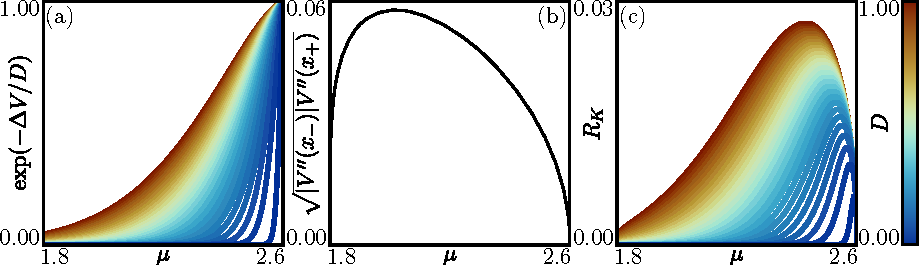
\includegraphics[keepaspectratio, width=\textwidth]{../figures/kramers_formula.pdf}
    \caption{Comparison of the modified escape early--warning signal \eqref{eq:escape_ews} (panel (a)) and Kramer's escape rate \eqref{eq:kramer_escape_formula} (panel (c)) at different values of the diffusion level $D$ (color-coded in the colorbar on the right).
            The prefactor term of Kramer's escape rate (panel (b)) is independent on $D$ and thus shown by a single black curve.}
    \label{fig:kramers_formula}
\end{figure}
%
On the other hand, setting $D=1$ guarantees that the modified formulation is not late in detecting the proximity of the tipping point whenever the underlying noisy fluctuations are small $D\to0$ (see Figure~\ref{fig:kramers_formula}(a)).
Furthermore, the true value of $D$ is generally not known a--priori and, while estimation is possible, it will inflate the dimensionality of the problem without providing significant advantages to the underlying detection of CSD.

The boundedness of \eqref{eq:escape_ews} in $(0,1]$ solves the interpretability problem we outlined above.
As opposed to the variance (and higher-order moments), a numerical value of the modified escape formula provides direct interpretation of the likelihood of a tipping event without the need for a baseline value to refer to.
If a system is far from a dangerous transition (i.e. $|\mu-\mu_c|\gg0\implies\Delta V\gg0$), then \eqref{eq:escape_ews} will be close to $0$; conversely, a state that is approaching said transition (i.e. $\mu\to\mu_c\implies\Delta V\to0$) results in values of the same quantity to be close to $1$.

In Figure~\ref{fig:escape_ews} we depict the monotonic increase of \eqref{eq:escape_ews} from $0$ to $1$ for May's model of ecosystem collapse we introduced in Chapter~\ref{chap:introduction}.
%
\begin{figure}[!t]
	      \centering
	      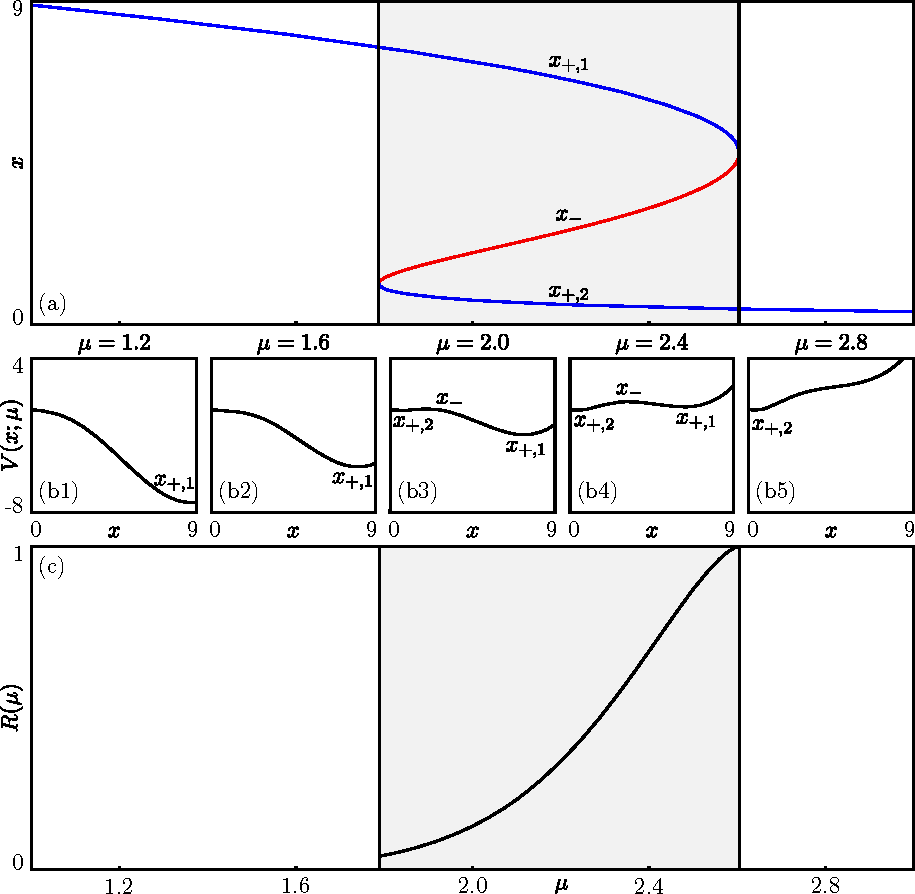
\includegraphics[keepaspectratio, width=\textwidth]{figures/escape_ews.pdf}
        \caption{(Panel (a)) Bifurcation diagram May's model of ecosystem collapse with the state $x$ (vegetation biomass) degrading as the forcing parameter $\mu$ (grazing rate) is increased. 
          Branches of stable equilibria ($x=x_{+,1}$ and $x={+,2}$) are in blue while the unstable branch ($x=x_-$) is in red; the region of bistability, bounded by two saddle--node bifurcations bifurcations, is shaded in gray.
        (Panels (b1-b5)) Different configurations of the potential $V(x;\mu) = -\frac{x^2}{2} + \frac{x^3}{30} + \mu\big(x - \arctan(x)\big)$ at different parameter values (ticks of the horizontal axes of panels (a) and (c)). 
        (Panel (c)) Modified escape early--warning signal \eqref{eq:escape_ews} computed out of the potential $V(x;\mu)$ between the stable state $x=x_{+,1}$ and the saddle $x=x_-$ within the bistability region.}
        \label{fig:escape_ews}
\end{figure}
%
The region of bistability (depicted by the gray area in Figure~\ref{fig:escape_ews} (a,c)) is bounded by two saddle--node bifurcations at $\mu_1$ and $\mu_2>\mu_1$.
The earlier saddle--node bifurcation at $\mu=\mu_1$ involves the (unhealthy) stable equilibrium $x=x_{+,2}$ and the unstable saddle $x=x_-$ while the later saddle--node bifurcation at $\mu=\mu_2$ involves the (healthy) stable equilibrium $x=x_{+,1}$ and the same saddle $x_-$.
This bifurcation sequence is reflected in the shape of the potential $V$ shown at a number of parameter slices in Figure~\ref{fig:escape_ews} (b1-b5), wherein the local maximum $x_-$ and the local minima $x_{+,1/2}$ correspond to the unstable and stable equilibria in Figure~\ref{fig:escape_ews} (a), respectively.
Outside the shaded region (i.e. $\mu<\mu_1$ or $\mu>\mu_2$, e.g. Figure~\ref{fig:escape_ews} (b1,b2,b5)) only one stable equilibrium exists (either $x_{+,1}$ or $x_{+,2}$), the potential $V$ has one global minimum and no local maxima and thus the modified escape EWS is undefined.
Conversely, inside the shaded region (i.e. $\mu_1<\mu<\mu_2$, e.g. Figure~\ref{fig:escape_ews} (b3,b4)) the potential $V$ has two minima $x_{+,1/2}$ and one local maximum $x_-$, meaning that the escape EWS can be computed using \eqref{eq:escape_ews} (e.g. Figure~\ref{fig:escape_ews} (c)).

Notice that the modified escape early--warning signal increases monotonically with $\mu$, with its minimum ($\exp(-\Delta V)\approx0$) being at $\mu=\mu_1$ and its maximum ($\exp(-\Delta V)=1$) being at $\mu=\mu_2$.
Therefore, by identifing the subset of the parameter space $\mathbb{R}$ such that $\Delta V$ has range $[0,+\infty)$, we associate to \eqref{eq:escape_ews} the intepretation of a probability measure, quantifying the likelihood of a tipping event to occur.
%
\section{Maximum likelihood estimation of the potential}\label{sec:mle}
Figure~\ref{fig:escape_ews} shows that \eqref{eq:escape_ews} can be used as an interpretable early--warning signal whenever the potential $V$ of a gradient system is known which, in most cases, it is not.
As mentioned above, the popularity of canonical early--warning signals, such as the increase in timeseries variance, is in part due to their simplicity in calculating them from available data.
In order for our proposed, interpretable early--warning signal to be applicable in the real--world we must be able to compute it from timeseries data without relying on prior knowledge of the system that generates it.

Since the modified escape rate \eqref{eq:escape_ews} depends on the potential barrier $\Delta V$ between the observed steady-state $x_+$ and an unknown unstable equilibrium $x_-$, our aim for this section is to estimate such quantity from a single timeseries. 
To do so we must be able to approximate the local shape of the potential $V(x;\mu)$ between $x_+$ and $x_-$.
As we are trying to infer the likelihood of a bifurcation--induced tipping, the minimum model that we can fit to a timeseries is that of a cubic polynomial $V(x;\theta) = \sum_{k=1}^{3}\theta_{k}x^{k}$ with real coefficients $\theta=(\theta_{1},\theta_{2},\theta_{3})$.
While different choices are available for our inference problem, a cubic polynomial is minimal in the sense that it allows for the presence of one local minimum $x_+$ and one local maximum $x_-$ (from which $\Delta V = V(x_-) - V(x_+)$ can be computed) without inflating the dimensionality of the search space.

The inference of the polynomial coefficients of the potential $V$ is, at its core, a parameter estimation problem of the deterministic drift of a SDE given a sequence of its realizations.
This is a well-established problem in statistical inference \cite[Ch. 11, p. 234]{Sarkka2019}; in the following we briefly formulate the setup for such problem and redirect interested readers to \cite{Nielsen2000, Sorensen2004, Craigmile2022} for reviews of these techniques.
%
\subsection{Problem formulation}\label{subsec:formulation}
A standard technique to infer the parameters of a model SDE, using its solution, is maximum likelihood estimation (MLE).
Suppose our sample $\mathcal{X}=\{X_{n}\}_{n=0,1,\dots,N}$ is made of $N+1$ observations of the stationary state solving Eq.~\eqref{eq:sde} from time $t=0$ to time $t=T$.
Suppose also that each observation is sampled at homogeneous frequency of time intervals $\Delta t = T/N$.
This It\^{o} process is a Markov process \cite[Ch.7, p. 111]{Oksendal2000} which means that the transition probability density to a future state $X_{t+1}$, at any time $t$, solely depends on the current state $X_{t}$ rather than the entire history $\mathcal{X}$.
This results in the joint distribution of the sample to be written in a factorized form of the (marginal) transition probability densities
%
\begin{equation}\label{eq:joint_distribution}
        p(\mathcal{X}) = p(X_{0})\prod_{n=1}^{N-1}p(X_{n+1}|X_{n})\,.
\end{equation}
%
From \eqref{eq:joint_distribution} we can define the likelihood of the sample to be generated by a parametrized transition density 
\begin{equation}\label{eq:likelihood_function}
        \mathcal{L}(\theta|\mathcal{X}) := p(X_{0}|\theta)\prod_{n=1}^{N-1}p(X_{n+1}|X_{n},\theta)\,,
\end{equation}
%
with parameters $\theta\in\mathbb{R}^p$.
By maximizing \eqref{eq:likelihood_function} one finds the most likely set of parameters $\theta^{*}$, for a family of transition densities $p(x|\theta)$, to have generated the observations $\mathcal{X} = \{X_{n}\}_{n=0,\dots,N}$.
Notably one reformulates this problem in the minimization of the inverse log-likelihood instead
%
\begin{equation}\label{eq:inv_log_likelihood}
        \ell(\theta|\mathcal{X}) = -\log\mathcal{L}(\theta|\mathcal{X}) \approx -\sum_{n=1}^{N-1}\log p(X_{n+1}|X_{n},\theta) \,,
\end{equation}
%
as this does not change the stationary point in the search space
%
\begin{equation}\label{eq:mle}
        \theta^{*}(\mathcal{X}) = \argmax_{\theta\in \mathbb{R}^{p}}\mathcal{L}(\theta|\mathcal{X}) = \argmin_{\theta\in \mathbb{R}^{p}}\ell(\theta|\mathcal{X})\,.
\end{equation}
%
Notice that in \eqref{eq:inv_log_likelihood} we approximate the inverse log-likelihhod by ignoring the conditional probability of the deterministic initial condition $X_{0}$ as this term is negligible compared to the sum of the log-likelihoods of the stochastic observations. 
The optimization problem \eqref{eq:inv_log_likelihood} requires the knowledge of the transition density $p(X_{n+1}|X_{n},\theta)$, which, for a SDE of the form \eqref{eq:sde}, is goverened by the Fokker-Plank equation \eqref{eq:fpe}, which can rarely be solved in closed form and often relies on analytical or numerical approximations.
%
\begin{figure}[t]
    \centering 
    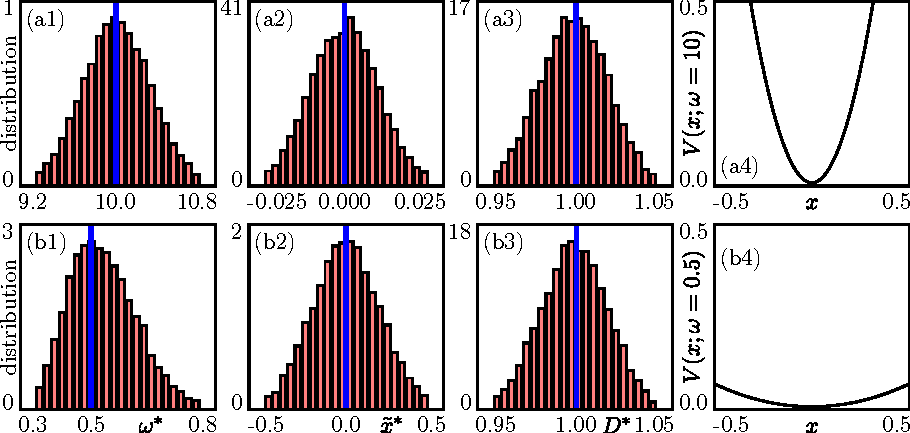
\includegraphics[keepaspectratio, width=\textwidth]{./figures/oup_mle.pdf}
    \caption{Distribution of the MLE of the parameters $\theta^* = (\alpha^*, x_+^*, D^*)$ of an ensemble of $10{,}000$ sample paths solving \eqref{eq:oup} for two different configurations of the potential $V(x) = \alpha(x_+ - x)^{2}$: a deep, strongly confining well with $\alpha = 10$ (panel (a4)) and; a shallow well with $\alpha = 0.5$ (panel (b4)).
            In each of the panels (a1-a3) and (b1-b3) the true value of the parameter is reported (blue line).
            Note, as $\alpha\to0$ the distribution of $\alpha^*$ becomes skewed despite the symmetry in the confining potential (panel (b1)).}
    \label{fig:oup_mle}
\end{figure}

\subsection{Time-invariant approximation: the Ornstein-Uhlenbeck process}\label{subsec:oup}
In the specific case of slow-fast systems of the form \eqref{eq:slow_fast}, the computation of the transition density can be simplified. 
Specifically, in the singular limit $\varepsilon\to0$ the (linear) ramp of the forcing parameter is much slower than the timescale of the evolution for the state variable. 
This means that the time-varying solution of Eq.~\eqref{eq:fpe} can be reasonably approximated with a time-invariant density $p(x|\theta)\approx p(x,t|\theta)$ by neglecting the (partial) time derivative $\partial_{t}p\approx0$ which, as established in \S~\ref{sec:stochastic_processes}, yields the equilibrium distribution \eqref{eq:stationary_fpe}.
Thus, in principle, one can use the time-invariant approximation \eqref{eq:stationary_fpe} as the transition density in the optimization problem \eqref{eq:mle}.

As an example of the applicability of this workflow, let us consider the simplified case of an Ornstein-Uhlenbeck process
%
\begin{equation}\label{eq:oup}
        dX_{t} = \alpha(x_+ - X_{t})dt + \sqrt{2D}dW_{t},
\end{equation}
%
where $\alpha,a> 0$.
By denoting $\theta=(\alpha,x_+,D)$ to be our parameter vector, we setup a MLE problem in which the (limiting) Gaussian distribtion of \eqref{eq:oup} is of Boltzmann-like form \eqref{eq:stationary_fpe} with quadratic potential $V(x) = \alpha(x_+ - x)^{2}$.
For large enough values of $\alpha$, the solution of this MLE problem has been shown to be asymptotically normal \cite{Sahalia2002}, as demonstrated in Figure~\ref{fig:oup_mle} (a1-a3).

When $\alpha\to0$ however, the distribution of $\alpha^*$ becomes skewed towards larger values (see Figure~\ref{fig:oup_mle} (b1)). 
On top of this, the standard deviation of the distribution of $x_+^*$ increases (see Figure~\ref{fig:oup_mle} (b2)), yielding an overall less accurate estimation.
Since we can interpret $\alpha=Df(x_+)$ to be the leading eigenvalue of the linearized vector field $f$ around the stable equilibrium $x_+$, we conclude that the MLE of a nonlinear SDE using the stationary distribution of the Ornstein-Uhlenbeck process decreases in accuracy as the tipping point is approached.
%
\subsection{Euler-Maruyama least-squares regression}\label{subsec:euler}
A desirable property of an early--warning signal is that its prediction becomes more accurate and reliable when the monitored system is in a proximity of the critical transition.
Conversly in fact, an early--warning signal that becomes less accurate when the system is close to tipping will systematically fail to detect the incoming critical transition by providing false negative outcomes, which has, arguably, a more catastrophic implication than providing false positive outcomes.
Estimating the likelihood of bifurcation--induced tipping using the transition density of the stationary Ornstein--Uhlenbeck process however achieves the opposite of this, as its accuracy decreases the closer the sample path is to the saddle--node bifurcation.
In this section we remedy and overcome this limitation by using an alternative approach to MLE.
To model bifurcation--induced tipping events of saddle--node type out of a sample path of \eqref{eq:slow_fast} we fit a cubic polynomial $V(x;\theta) = \sum_{k=1}^{3}\theta_{k}x^{k}$ to its potential.

A number of computational methods to approximate the stationary density $p(x)$ are available \cite{Pedersen1995, Jensen2002, Sahalia2002}.
Conversely, other techniques have been devised that do not rely on the numerical approximation of the transition density such as the generalized method of moments \cite{Hansen1982}, Markov chain Monte-Carlo algorithms \cite{Roberts2001,Alexander2005} and quasi--maximum likelihood regressions \cite{Castelle1986, Yoshida1992}.
Here we focus on the latter approach and in particular we describe one quasi--maximum likelihood technique that reduces the MLE problem into an ordinary least--squares regression.

As usual, we assume our sample path $\mathcal{X} = \{X_{0},\dots,X_{N}\}$ to be a solution of \eqref{eq:sde} under the stationarity restriction.
We can then approximate the entire sample path using the Euler-Maruyama time--stepping scheme, which is a generalization to stochastic processes of the Euler method for ordinary differential equations.
This defines a stochatic iterated map of the form
%
\begin{equation}\label{eq:euler_maruyama}
        X_{n+1} = X_{n} -V'(X_{n};\theta)\Delta t + \sqrt{2D\Delta t}\,\xi\,,\quad \xi\sim\mathcal{N}(0,1)\,,
\end{equation}
%
where $\theta=(\theta_1,\theta_2,\theta_3)\in\mathbb{R}^{3}$ is the vector of polynomial coefficients parameterizing the cubic potential.
We rearrange Eq.~\eqref{eq:euler_maruyama} to define the first-order time increments
%
\begin{equation}\label{eq:increments}
        Y_{n} := \frac{X_{n+1} - X_{n}}{\Delta t} = -V'(X_{n};\theta) + \sqrt{\frac{2D}{\Delta t}}\,\xi = -V'(X_{n};\theta) + \Xi\,,\quad\Xi\sim\mathcal{N}\bigg(0,\frac{2D}{\Delta t}\bigg)\,.
\end{equation}
%
Notice now how \eqref{eq:increments} defines a regression to a model $V'$ of some data $\{X_{n}\}_{n=0,\dots,N-1}$ given a set of $N$ observations $\{Y_{n}\}_{n=0,\dots,N-1}$ perturbed by some Gaussian noise $\Xi$.
This sets up a parameter estimation problem in which one wishes to find an optimal parametrization $\theta^*$ of the potential such that the residual between the model predictions $V'(X_{n};\theta^*)$ and the observations $Y_{n}$ is minimized in some sense.
As anticipated above, we formulate an ordinary least--squares problem by interpreting the noise $\Xi$ to be unresolved fluctuation errors in the observed data.
We thus minimize the residual vector
%
\begin{equation}\label{eq:residual}
        r(\theta) = \big(Y_{n} + V'(X_{n};\theta)\big)_{n=1,\dots,N-1}\,,
\end{equation}
%
between the observations $Y_n$ and the fitting model $V'(X_n,\theta)$ in the least--squares sense.
That is, we solve the minimization problem
%
\begin{equation}\label{eq:lls_problem}
        \theta^{*} = \argmin_{\theta\in \mathbb{R}^{3}}||r(\theta)||_{2}\,,
\end{equation}
%
where $||\cdot||_2$ denotes the $L_2-$norm.
%
\begin{algorithm}[!t]
        \DontPrintSemicolon
        \SetAlgoNoLine
        \SetAlgoNlRelativeSize{0}
        \SetNlSty{text}{\Indp}{.}
        \SetKwInput{Input}{Input}
        \SetKwInput{Output}{Output}
        %
        \BlankLine 
        %
        \Input{sample $\mathcal{X}=\{X_0,X_1,\dots,X_N\}$ (a single timeseries)}
        \Output{estimated likelihood of tipping}
        %
        \BlankLine 
        \hrule
        \BlankLine
        %
        \nl Compute quasi-stationary residuals $\overline{\mathcal{X}}$ using a detrending technique.
        \BlankLine
        %
        \nl Assemble the ordinary least--squares problem \eqref{eq:increments}\;
        \Indp\For{$(X_n,X_{n+1})\in \overline{\mathcal{X}}$}{
                \vspace{-10pt}
                \begin{align*}
                        y_n &= X_{n+1} - X_n\,,\\
                        A_n &= \big(X_n,\;X_n^2,\;X_n^3\big)\,.
                \end{align*}
                \vspace{-20pt}
        }
        \Indm\BlankLine
        %
        \nl Solve the normal equation \eqref{eq:lls_solution}
        \begin{equation*}
                \theta^* = (\theta^*_1, \theta^*_2, \theta^*_3) = (A^TA)^{-1}A^Ty\,.
        \end{equation*}
        \BlankLine
        %
        \nl Compute the local minimum and local maximum of $V^*(x)=\sum_{k=1}^{3}\theta_k^*x^k$
        \begin{align*}
                x_{\text{min}} &= + \frac{1}{3\theta^*_3}\bigg(\sqrt{(\theta_2^*)^2 - 3\theta_1^*\theta_3^*} - \theta^*_2\bigg)\,,\\
                x_{\text{max}} &= - \frac{1}{3\theta^*_3}\bigg(\sqrt{(\theta_2^*)^2 - 3\theta_1^*\theta_3^*} + \theta^*_2\bigg)\,.
        \end{align*}
        \BlankLine
        %
        \nl Compute the potential barrier 
        \begin{equation*}
                \Delta V^*=V^*(x_{\text{max}}) - V^*(x_{\text{min}})\,.
        \end{equation*}
        \BlankLine
        %
        \nl Extract the modified escape early--warning signal using Eq.~\eqref{eq:escape_ews}
        \begin{equation*}
                \text{EWS} = \exp(-\Delta V^*)\,.
        \end{equation*}
        \vspace{-10pt}
        \caption{Computation of an interpretable early--warning signal from timeseries.}
        \label{alg:modified_ews}
\end{algorithm}
%
Notice that by fitting the minimal working model of B-tipping (i.e. we assume $V(x;\theta)$ is a cubic polynomial of coefficients $\theta = (\theta_{1},\, \theta_{2},\, \theta_{3})$), the residual \eqref{eq:residual} is linear in $\theta$.
%
\begin{figure}[!t]
    \centering 
    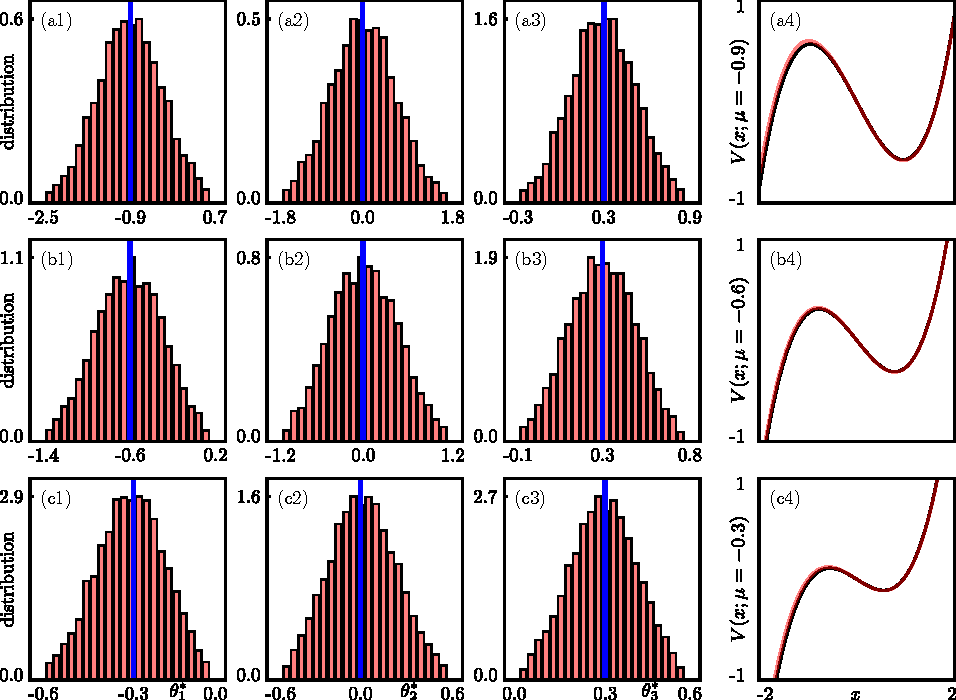
\includegraphics[keepaspectratio, width=\textwidth]{./figures/lls_solutions.pdf}
    \caption{Distribution of the solutions $\theta^{*} = (\theta_{1}^{*},\,\theta_{2}^{*},\,\theta_{3}^{*})$ of the ordinary least--squares problem \eqref{eq:lls_solution} for an ensemble of $5{,}000$ sample paths of a saddle--node normal form $f(x;\mu) = -\mu - x^2$.
            The problem is solved for different configurations of the potential $V(x;\mu) = \mu x + \frac{x^3}{3}$; at $\mu = -0.9$ (panels (a1-a4)), $\mu=-0.6$ (b1-b4) and $\mu=-0.3$ (c1-c4).
            The value of the polynomial coefficients of the true potential are reported in each of the panels (a1-a3), (b1-b3) and (c1-c3) (blue line).
            The ensemble mean values of the least--squares solutions $\hat{\theta}^{*} = (\hat{\theta}_{1}^{*},\,\hat{\theta}_{2}^{*},\,\hat{\theta}_{3}^{*})$ are used to plot an ensemble mean reconstruction (red curve in (a4-c4)) of the potential $\hat{V}^{*}(x) := V(x;\hat{\theta}^{*}) = \sum_{k=1}^{3}\hat{\theta}_{k}^{*}x^{k}$ and compared with the ground truth (black curve in (a4-c4)).}
    \label{fig:lls_solutions}
\end{figure}
%
This allows us to rewrite \eqref{eq:lls_problem} as a minimization problem on the quadratic form quadratic 
%
\begin{equation}\label{eq:quadratic_minimization_problem}
        \theta^{*} = \argmin_{\theta\in \mathbb{R}^{3}}||A\theta - y||_2\,,
\end{equation}
%
where $y\in \mathbb{R}^{N}$ denotes the observation data vector (i.e. $y_j = Y_j$), $A\in \mathbb{R}^{N\times3}$ is the model matrix evaluated on the sample $\mathcal{X}$ (i.e. $A_{jk} = X_{j}^{k}$) and $A\theta - y = r(\theta) \neq 0$.
The unique solution of \eqref{eq:quadratic_minimization_problem} satisfies the so-called normal equation
%
\begin{equation}\label{eq:lls_solution}
        \theta^{*} = (A^{T}A)^{-1}A^{T}y = A^{+}y\,,
\end{equation}
%
where $A^TA$ is a Gram matrix and $A^{+}\in\mathbb{R}^{3\times N}$ is the Moore-Penrose inverse of $A$.

With the estimation $\theta^*=(\theta^*_1, \theta^*_2, \theta^*_3)$ one can readily compute the modified escape early--warning \eqref{eq:escape_ews} of the approximation $V^*(x):=V(x;\theta^*)$ using the sample path. We report the main steps of this procedure in Algorithm~\ref{alg:modified_ews}.
The solution of the normal equation \eqref{eq:lls_solution} is also asymptotically normal as shown in Figure~\ref{fig:lls_solutions}.

Notice that, contrary to the MLE using the stationary density of the Ornstein--Uhlenbeck process described in \S~\ref{subsec:oup}, the numerical accuracy of \eqref{eq:lls_solution} improves as the saddle--node bifurcation is approached.
This is shown in Figure~\ref{fig:lls_solutions} by a reduction of the standard deviation of the distribution (histograms) of the least--squares solutions $\theta^*$ as $\mu\to0$.
We remark that this property is generic (i.e. it is observed for gradient systems other than the saddle--node normal form); we argue that is is a desirable consequence of CSD.
As tipping is approached (i.e. $\mu\to0$) the leading eigenvalue of the linearized system approaches $0$ from below, which in turn entails that the stable equilibrium recovers perturbations of the steady--state with less \emph{``strength''}.
With the fluctuations around the stable equilibrium $x_+$ increasing in range, the state of the system will explore larger portions of the basin of attraction of such equilibrium.
As a consequence, the realizations $\mathcal{X} = \{X_0,\dots,X_N\}$ of the gradient system will capture the local shape of the confining potential in an increasingly better fashion as the system is driven closer to the tipping, which translates in more accurate solutions of the regression \eqref{eq:lls_solution}.

\section{Performance analysis}\label{sec:analysis}
The derived pipeline in Algorithm~\ref{alg:modified_ews} shows that the modified escape EWS can, in principle, be estimated from slowly varying timeseries following the MLE of the potential discussed in \S~\ref{sec:mle}.
However, the statistical significance and uncertainties associated with such method can be heavily affected by the timescale separation $0<\varepsilon\ll1$, noise intensity $0<\sigma<1$, sampling frequency $0<\Delta T<1$ and sample lengths $N\gg0$.
In the following section we investigate how the performance of the proposed inference method is affected by varying these parameters.
We thus perform statistical analysis of the relevant quantities involved in the estimation of the modified escape early--warning signal following Algorithm~\ref{alg:modified_ews}.
As a representative example, we consider a one-dimensional, slow--fast system of the form
%
\begin{equation}
        \begin{aligned}\label{eq:bistable_model}
                dX_t &= (-\mu + 4x - 4x^3)dt + \sigma dW_t\,,\\ 
                d\mu &= \varepsilon dt\,,
        \end{aligned}
\end{equation}
%
where the bistable drift $f(x,\mu)= -\mu + 4x - 4x^3$ undergoes a saddle--node bifurcation at $\mu_c\approx1.53$.

\subsection{Robustness of the residuals}\label{subsec:residuals}

\begin{figure}[t]
    \centering 
    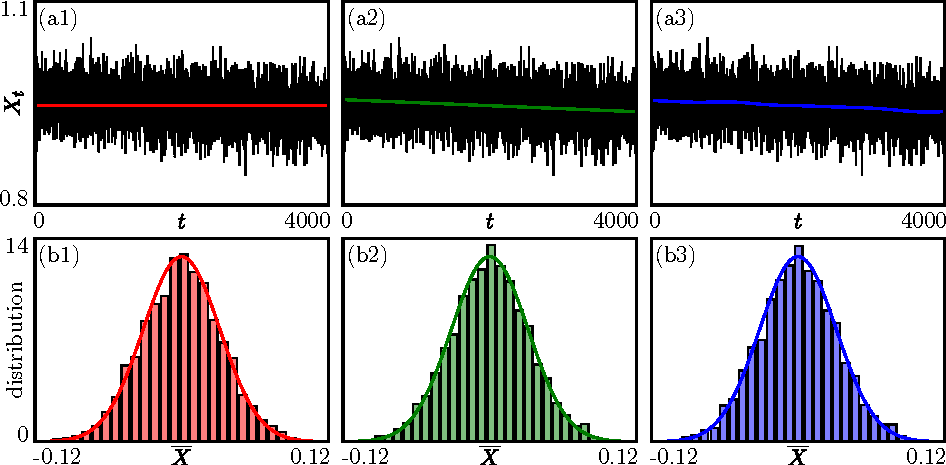
\includegraphics[keepaspectratio, width=\textwidth]{./figures/residuals_distribution.pdf}
    \caption{Comparison of detrending techniques for a solution $\mathcal{X}$ of \eqref{eq:bistable_model} with $\mu_0=0$, $\varepsilon=5\cdot10^{-4}$ and $\sigma=0.1$; the simulation stops at the parameter value $\mu(T)=0.2$.
            Panels (a1-a3): trends for the same ramped timeseries (black curves) are computed using the sample mean (red curve), linear fit (green curve) and EMD (blue).
            Panels (b1-b3): comparison between the stationary density of the OUP approximating $\mathcal{X}$ (colored curves) and the empirical distribution of the residuals obtained by sample mean removal (red histogram), linear fit (green histogram) and EMD (blue histogram).}
    \label{fig:residuals_distribution}
\end{figure}

One of the assumptions of the MLE of the modified escape early--warning signal is that the underlying distribution of the sample path is stationary.
However, solutions $\mathcal{X} = \{X_0,\dots,X_N\}$ of slowly ramped systems, such as \eqref{eq:bistable_model}, only satisfy this condition in the singular limit $\varepsilon\to0$ and for long enough time horizons $N\to\infty$.
For strictly positive rates $\varepsilon>0$ the deterministic drift $f$ is nonautonomous and thus the FPE of the system does not admit a Boltzmann-like stationary solution \eqref{eq:stationary_fpe}.
Nonetheless, by considering slow-fast regimes for which $0<\varepsilon\ll1$, we can obtain a quasi-stationary sample $\overline{\mathcal{X}}=\{\overline{X}_1,\dots,\overline{X}_N\}$ by removing the underlying trend in the ramped sample path $\mathcal{X}$.
The detrending of non-stationary timeseries (see step 1. in Algorithm~\ref{alg:modified_ews}) is a fundamental pre-processing stage in the derivation and analysis of early--warning signals as the quality of the extracted quasi-stationary residuals can affect the performace of the estimation.

One method to do that is the Empirical Mode Decomposition (EMD) \cite{Huang1998} which is a data-driven technique that extracts the underlying trend of a timeseries through a sifting procedure.
Specifically, EMD iteratively decomposes a timeseries in so-called Intrinsic Mode Functions (IMFs), each capturing the different scales of fluctuations in the timeseries.
The trend of a sample path $\mathcal{X}$ thus corresponds to the IMF with the largest scale of fluctuation (see \cite{Huang1998} for details) and the residuals $\overline{\mathcal{X}}$ are obtained by removing the leading IMF from the sample path.

A desirable property of EMD is that it does not require fine calibrations as the IMFs are extractred through the envelopes of the timeseries.
This makes the application of EMD particularly suitable in the computation of quasi-stationary residuals $\overline{\mathcal{X}}$ as it readily extends to univariate timeseries with generic trends without the need of fine-tuning additional parameters.
Similar data-driven techniques, often used in applications, are centering (i.e. removal of the sample mean from the timeseries) and linear fit (i.e. removal of the slope from the timeseries).

We simulate an ensemble of $1{,}000$ sample paths of \eqref{eq:bistable_model} ramped between $\mu_0=0.0$ and $\mu(T)=0.2$ with $\varepsilon=5\cdot10^{-4}$; for each of those sample paths we apply detrending by EMD, linear fit and centering and analyse the residuals separately.
In order to assess the quality of the obtained residuals with respect to the stationary assumption, an OUP, approximating the slowly ramped sample paths, is constructed with coefficients $\alpha=Df(x_+)$ and $x_+$ being evaluated at $\mu(T)=0.2$ (see Eq.~\eqref{eq:oup}).

Figure~\ref{fig:residuals_distribution} shows a representative example of this experiment where a sample path of the simulated ensemble (black curves in panels (a1-a3)) is detrended by centering (red curve, panel (a1)), linear fit (green curve, panel (a2)) and EMD (blue curve, panel (a3)).
The distribution of the quasi-stationary residuals (histograms in panels (b1-b3)) are then compared to the stationary distribution of the OUP (see Eq.~\eqref{eq:oup_density}).
To quantify the deviation of the residuals from the stationary assumption we compute the relative error between the residuals' statistics $\overline{q}_k$ and the central moment $q_k$ of the OUP
%
\begin{equation}\label{eq:relative_error}
        E_k\coloneqq \frac{|\overline{q}_k - q_k|}{|q_k|}\,,
\end{equation}
%
where $k=1,2,3$ denote the first (mean), second (variance) and third (skewness) moment of the distribution.
The results of this experiment, compiled in Table~\ref{tab:relative_error}, show that, within the slow ramp regime $0<\varepsilon\ll1$, the three detrending techniques largely preserve the stationary assumption in their residuals with average relative errors well within $10\%$.
%
\begin{table}[t]
    \centering
    \caption{Relative errors statistics \eqref{eq:relative_error} of an ensemble of $1{,}000$ residuals obtained by different detrending techniques.}
    \label{tab:relative_error}
    \footnotesize
    \setlength{\tabcolsep}{3pt}
    \begin{tabular*}{\textwidth}{@{\extracolsep{\fill}} l ccc ccc ccc @{}}
    \toprule
    & \multicolumn{3}{c}{Centering}
    & \multicolumn{3}{c}{Linear fit}
    & \multicolumn{3}{c}{EMD} \\
    \cmidrule(lr){2-4}
    \cmidrule(lr){5-7}
    \cmidrule(lr){8-10}
    & min & mean & max & min & mean & max & min & mean & max \\
    \midrule
    $E_1$ & $5\cdot10^{-19}$ & $4\cdot10^{-17}$ & $4\cdot10^{-16}$ & $5\cdot10^{-19}$ & $1\cdot10^{-16}$ & $6\cdot10^{-16}$ & $2\cdot10^{-6}$ & $3\cdot10^{-4}$ & $2\cdot10^{-3}$ \\
    $E_2$ & $0.02$ & $0.03$ & $0.05$ & $0.03$ & $0.04$ & $0.05$ & $0.03$ & $0.04$ & $0.05$ \\
    $E_3$ & $2\cdot10^{-5}$ & $0.03$ & $0.16$ & $6\cdot10^{-5}$ & $0.03$ & $0.19$ & $1\cdot10^{-4}$ & $0.03$ & $0.18$ \\
    \bottomrule
    \end{tabular*}
\end{table}
%
Notice that, while the three techniques yield similar residuals, EMD has the advantage of generalising to more complex and nonlinear transient regimes beyond the slow ramp forcing considered throughout this manuscript.

\subsection{Accuracy and sensitivity}\label{subsec:sensitivity}
The statistical properties of the least--squares solutions are prescribed by the normally distributed uncertainties $\Xi\sim\mathcal{N}(0,\sigma^2/\Delta t)$ in the first-order increments (see Eq.~\eqref{eq:increments}).
As a result, the accuracy of the least--squares solutions, and hence the MLE of the modified escape early--warning signal, are reflected by the specific choices of additive noise intensity $\sigma$ and sampling frequency $\Delta t$.
Furthermore, it is reasonable to expect that shorter (i.e. smaller $N$) and faster (i.e. larger $\varepsilon$) timeseries would produce significantly different residuals and thus hinder the stationary assumption discussed above. 

We investigate the sensitivity of the MLE of the modified escape early--warning signal when the above constraints (long and slow timeseries with small noise and large sampling frequency) are relaxed.
Specifically, we test the accuracy of Algorithm~\ref{alg:modified_ews} in two different settings:
%
\begin{itemize}
     \item by varying the timeseries length $N$ and sampling frequency $\Delta t$ in the singular limit $\varepsilon\to0$ and in a regime of small noise $\sigma\to0$ and;
     \item by varying the parameter's rate of change $\varepsilon$ and noise level $\sigma$ with fixed timeseries length $N$ and sampling frequency $\Delta t$.
\end{itemize}
%
In both cases we run an ensemble simulation of $1{,}000$ sample paths of \eqref{eq:bistable_model} and evaluate the accuracy of the proposed method by computing the a-posteriori relative error (see Eq.~\eqref{eq:relative_error}) between the estimated modified escape early--warning signal and the ground truth.
In order to assess whether the convergence in mean persists in different regimes, we compare the relative errors at different parameter values as the system is driven closer to tipping (i.e. as $\mu\to\mu_c$).
 
The results of this experiment are depicted in Figure~\ref{fig:statistical_performance}.
%
\begin{figure}[!t]
    \centering 
    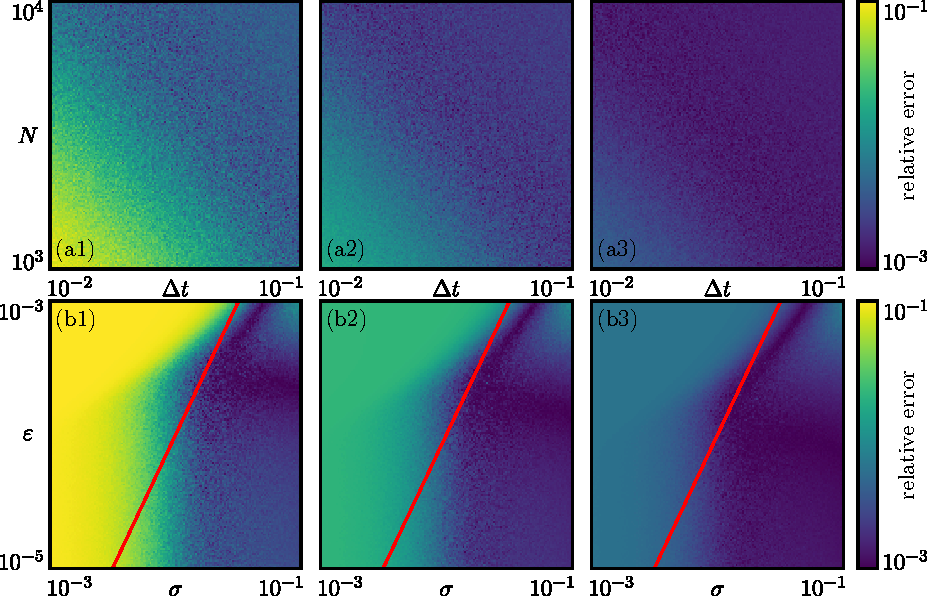
\includegraphics[keepaspectratio, width=\textwidth]{./figures/statistical_performance.pdf}
    \caption{Sensitivity of the relative error of the MLE modified escape early--warning signal under different regimes.
            Each pixel in the heatmap corresponds to the ensemble mean relative error of $1{,}000$ sample paths of \eqref{eq:bistable_model}.
            Panels (a1-a3): in the stationary case ($\varepsilon=0$) and with fixed small noise ($\sigma=0.05$) longer timeseries, sampled at larger frequencies, yield a more accurate estimation of the modified escape EWS.
            Panels (b1-b3): in the slow-fast regime, for fixed timeseries length $N=10{,}000$ and sampling frequency $\Delta t = 0.1$, the accuracy of the estimated modified escape early--warning signal depends, non-trivially, from the level of additive noise in the system with smaller noise seemingly yielding less accurate estimations.
            The red curve represents the $\sigma=\sqrt{\varepsilon}$ threshold.}
    \label{fig:statistical_performance}
\end{figure}
%
In the stationary case (panels (a1-a3)) we observe that the modified escape early--warning signal estimate is more accurate for longer timeseries $N\to10^4$ and larger sampling frequencies $\Delta t\to10^{-1}$.
This is not surprising considering that the uncertainty in the ordinary least--squares regression is inversely proportional to $\Delta t$.
Furthermore, we notice that the increase in accuracy close to tipping is preserved for varying $N$ and $\Delta t$ as the mean relative error for the system far from the saddle--node bifurcation $\mu=1.1$ (panel (a1)) is overall larger than the one for the system closer to the saddle--node bifurcation $\mu=1.3$ (panel (a3)).
In the slow-fast regime (panels (b1-b3)) we keep the timeseries length $N=10^4$ and sampling frequency $\Delta t=10^{-1}$ fixed while we generate solutions of \eqref{eq:bistable_model} at varying rates $\varepsilon$ and noise intensities $\sigma$.
For each $\varepsilon$ we keep $\mu(T)$ fixed and adjust $\mu_0$ so that each sample path contains exactly $N=10^4$ realizations.
In particular $\mu(T)\in\{1.1,1.2,1.3\}$ in panels (b1), (b2) and (b3) respectively; these parameter values are then used to compute the ground truth of the modified escape early--warning signal.
Intuitively, we observe that faster rates $\varepsilon\to10^{-3}$ yield overall less accurate estimations due to the residuals deviating further from the stationary assumption (as discussed in the previous section).
On the other hand, the estimations become less accurate for smaller noise levels $\sigma\to10^{-3}$; while Kramer's law holds in regimes of small noise, the least--squares estimation of the confining potential requires larger excursions around the stable equilibrium to better infer the local shape of the basin of attraction.
In particular, we notice that the non-trivial decay of the relative error shows a complex relationship modelling the interplay of $\varepsilon$ and $\sigma$ in different regimes, meaning that slower and less noisy timeseries do not necessarly yield better estimates.
This emphasizes the fact that the MLE of the modified escape early--warning signal is sensitive to perturbations in forced systems and in particular how the threshold $\sigma=\sqrt{\varepsilon}$ (red curves in panels (b1-b3)), separating regimes of slow passage through bifurcation--induced tipping from noise--induced escapes, provides an actionable guideline for applications.

\subsection{Statistical significance}\label{subsec:significance}
\begin{figure}[!t]
    \centering 
    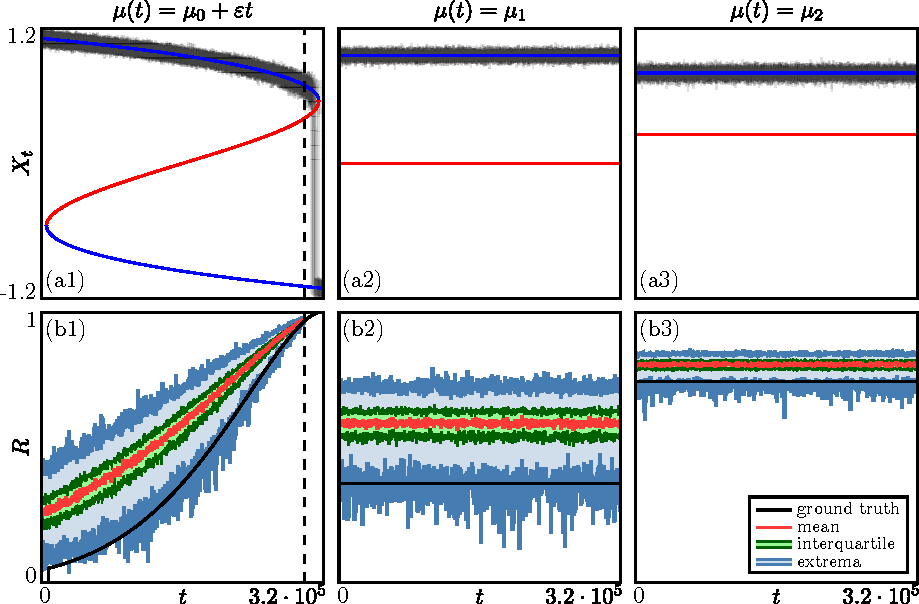
\includegraphics[keepaspectratio, width=\textwidth]{./figures/statistical_significance.pdf}
    \caption{Time-varying estimations of the modified escape early--warning signal for an enseble $1{,}000$ slowly ramped (panels (a1)-(b1)) and stationary (panels (a2-a3)-(b2-b3)) solutions of \eqref{eq:bistable_model}.
            In the ramped case the parameter varies between $\mu_0=-1.6$ to $\mu(T)=1.6$ with rate $\varepsilon=1\cdot10^{-5}$. 
            The sample paths, shown by the black curves in panel (a1), follow the upper stable branch of the bifurcation diagram (blue curve) of the frozen system before tipping across the unstable branch (red curve).
            The earliest tipping in the ensemble is indicated by the vertical dashed line.
            In the stationary cases the system is in the singular limit $\varepsilon\to0$ and thus the solutions, shown by the black curves in panels (a2-a3), are confined around the stable equilibrium (blue line) and do not tip across the unstable equilibrium (red curve) within the simulated time horizon.
            The stationary cases are simulated at parameter values $\mu=0$ (panel (a2)) and $\mu=1$ (panel (a3)).
            In all cases, a rolling window of $10\%$ the length of the sample paths, is used to estimate the modified escape EWS of the entire ensemble (panels (b1-b3)).
            The ensemble envelope (i.e. maximum and minimum values) of the estimations are depicted by the blue shaded regions, whereas the interquartile range is depicted by the green shaded regions. 
            The ensemble mean is shown by the red curves and it is compared with the ground truth of the frozen system, depicted by the black curves.}
    \label{fig:statistical_significance}
\end{figure}
%
The convergence in mean of the estimated modified escape early--warning signal guarantees accurate warnings when an ensemble of sample paths is available.
In real-world applications however, this is rarely the case as access to i.i.d. samples of a given system is limited by physical and technical constraints.
We therefore investigate how significant the upward trend for the estimated modified escape early--warning signal is for individual realizations of \eqref{eq:bistable_model}.
In particular, we are interested in establishing whether the estimations from single sample paths can lead to missed allarms (i.e. false negatives) and/or spurious warnings (i.e. false positives).

To do so we perform an ensemble simulation of $1{,}000$ sample paths ramped from $\mu_0=-1.6$ to $\mu(T)=\mu_c$ with $\varepsilon=1\cdot10^{-5}$.
We then use Algorithm~\ref{alg:modified_ews} to estimate the modified escape early--warning signal across a sliding window containing $N=10^4$ realizations of each sample path.
We repeat the same procedure for stationary simulations of \eqref{eq:bistable_model} at parameter values $\mu_1=0$ (i.e. at a safe distance from tipping) and $\mu_2=1$ (closer to tipping but still at a safe distance).
We report the results of this analysis in Figure~\ref{fig:statistical_significance}.
The sample paths (black curves in panels (a1-a3)) are computed across a time horizon $T=3.2\cdot10^5$. 
For the slowly ramped case (panel (a1)), the timeseries will all tip, from the drifting stable equilibrium (blue curves), across the unstable threshold (red curve), within the prescribed time horizon; this provides a sample of positive tipping events.
For the stationary cases (panels (a2-a3)) the solutions will stay bounded around a small region of the stable equilibrium (blue line) and they will not tip across the unstable threshold (red line) within the time horizon (red line); this provides a sample of negative tipping events.
In the ramped case, the estimated ensemble mean of the modified escape early--warning signal (red curve, panel (b1)) overestimates the proximity to tipping given by the ground truth (black curve) partly due to less amount of data available; notice that the familiar convergence in mean, as $\mu\to\mu_c$, implies that the overestimation bias vanishes close to tipping.
Furthermore, while the interquartile range (green shaded region) shows a reasonable bounded region for the estimated signal, the outliers in the ensemble (blue shaded region) deviate significantly from the mean.
This feature of the MLE of the modified escape early--warning signal is also observed in the stationary cases with the deviations reducing as the system is driven closer to tipping.

We conclude that, the overestimation bias in the ensemble mean, and the large deviations of the outliers from such mean can lead to spurious warnings when a single trajectory is considered.
However, considering that the interquartile range provides a considerably smaller region around the mean, and that such deviations vanish as $\mu\to\mu_c$, we can also conclude that the overall trends of the estimations become more significant as the system approaches the saddle--node bifurcation, which minimizes the occurence of missed alarms from single trajectories.
Notice that, variability in the outliers of the estimated early--warning signal can be alleviated by considering moving averages of the timeseries, thus yielding much more reliable indicators that can also minimize spurious warnings.
